
\chapter{Autonomous Aerial Refueling of Multiple Receivers: An Efficient Rendezvous Scheduling Approach}

Autonomous aerial refueling (AAR) is an important capability for the future successful deployment and operation of unmanned aerial vehicles (UAVs), so it is necessary to design an efficient rendezvous scheduling approach. In this paper, a general strategy for refueling missions is proposed for intensive refueling firstly, and then the tanker flight path and virtual queue sequence points are designed. Secondly, to obtain the optimal refueling time under the strategy, an integer linear programming (ILP) algorithm based on the branch-and-bound method is proposed, and some planning is further made for the waiting queue adjustment. Finally, the effectiveness of the proposed approach is demonstrated by simulation via two indexes, namely, the minimum oil volume and average volume of the receivers at the start of  the refueling.

\section{Introduction}
UAVs have been widely used in recent years, however, their navigation time is limited by the rate of fuel consumption, so they mainly perform limited search and reconnaissance missions, which makes the study of autonomous aerial refueling technology for UAVs an urgent need, as recently verified by the first successful U.S. refueling mission of the MQ-25 Stingray unmanned refueling aircraft as shown in Fig. 1. Besides, UAVs have developed toward fleeting and clustering, relying on effective collaboration to solve complex missions, which requires autonomous aerial refueling technology for multiple UAVs \cite{b1}.
\begin{figure}[htbp]
	\centerline{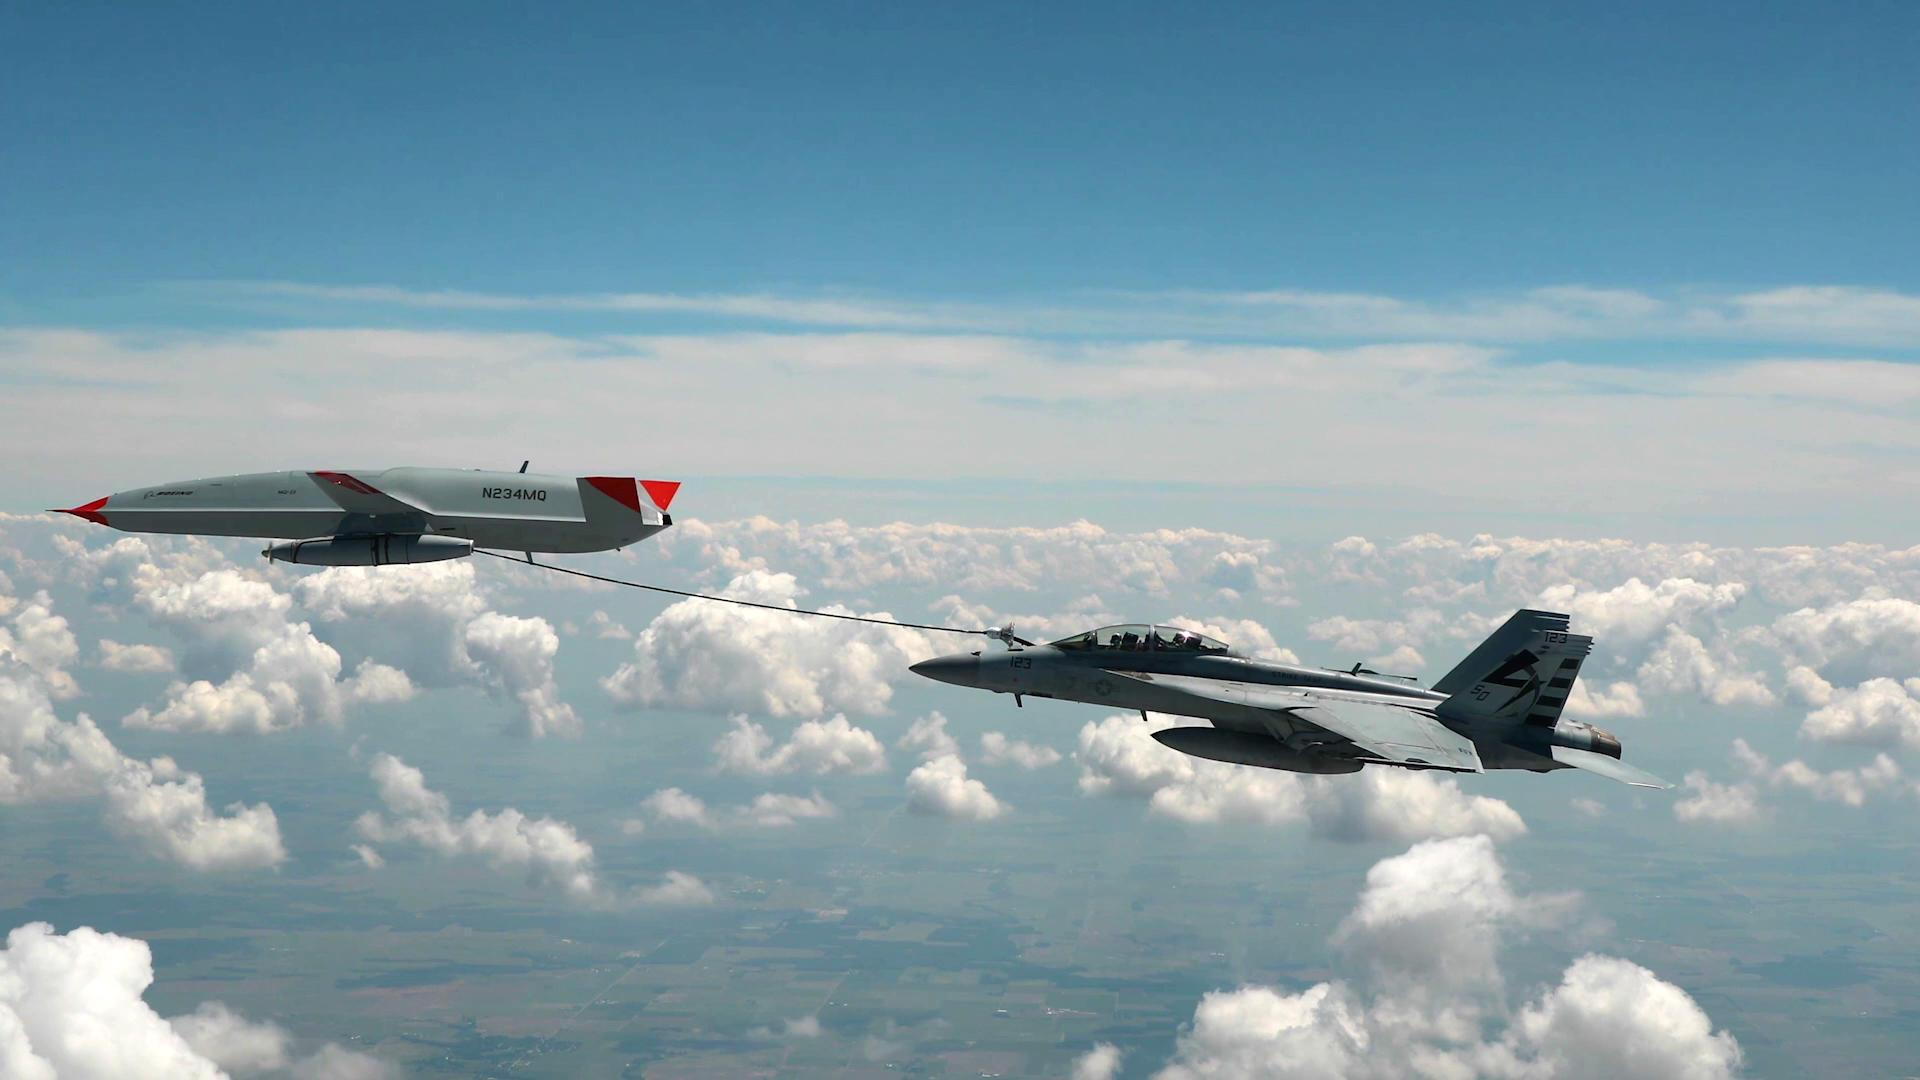
\includegraphics[width=.45\textwidth]{Figures/Figs_Ch15/05bc5d138937a5b023e613758ee9b368.jpg}}
	\caption{Drone refuels U.S. Navy fighter jet in midair for the first time.}
	\label{fig}
\end{figure}

The rendezvous is a prerequisite for aerial refueling; much researches have focused on the one-to-one rendezvous between a single receiver and a single tanker \cite{b3,b4,b5,b6}. The main rendezvous strategies currently include on-course, point parallel, and en-path rendezvous \cite{b2}. Point parallel requires the receiver to be at the refueling control point in advance, and en-path strategy requires that the tanker and receiver arrive at the rendezvous point simultaneously, forming a co-linear formation. A rendezvous path between a tanker and a receiver on the intended path to achieve rendezvous in the shortest time \cite{b3,b4}. A vector field-based 3D convergent path design method was proposed based on the Dubins model \cite{b5}. A heuristic search algorithm was designed based on a tanker flight path \cite{b6}. The problem of one-to-one rendezvous between a single tanker and a single receiver lacks the adaptability to the complex air traffic environment in the future. In \cite{b7}, virtual points and tanker's path are designed to achieve multiple receiver refueling and saving fuel by preventing the receiver from hovering in the air. 

However, there still exist some challenges in the path planning for aerial refueling of multiple receivers.
First of all, the influence of the complexity of the UAV missions on the refueling task is not considered.
For example, the refueling order of the UAVs who perform reconnaissance missions may be higher than that who execute the attacking missions. 
On the other hand, it is now mainly considered to expand the path of the tanker to complete the refueling of multiple UAVs, the safety of the refueling aircraft is difficult to ensure. 
Last but not least, the refueling interval between UAVs is considered relatively large for UAV formation. In the case of UAVs departing in formation for an assignment, which means that the refueling interval of the receiver is relatively small, how to complete refueling safely and efficiently has not been considered.

To solve the mentioned problems, this study proposes a novel path design for both  tankers and receivers. The proposed strategy limits the fly range of the tanker and design a waiting queue for receivers. This is suitable for solving the intensive time refueling problem under a specific refueling sequence and guarantees the aircraft safety. Besides, based on the path, to get the minimum time consumption, a target point assignment algorithm for each receiver is proposed and some rules are made when the receivers are waiting in the queue.

This paper is organized as follows. The designed tanker's path and the whole refueling task procedures are introduced in Sec. \uppercase\expandafter{\romannumeral2}. In Sec. \uppercase\expandafter{\romannumeral3}, the problem is analyzed. Then, in Sec. \uppercase\expandafter{\romannumeral4}, the main algorithm used in this paper is presented. Then, in Sec. \uppercase\expandafter{\romannumeral5}, the details and results of the simulation are presented. Finally, in Sec. \uppercase\expandafter{\romannumeral6}, the conclusions are drawn. 

\section{Refueling Task Strategy and Problem Formulation}
The tanker's path and virtual queue sequence points for receivers are specially designed and introduced in this part. Based on the path, the whole procedure of the refueling task in this paper is introduced and the problem is formulated.

\subsection{Tanker's Path and Virtual Queue Sequence Points Design}

\begin{figure}[htbp]
	\centerline{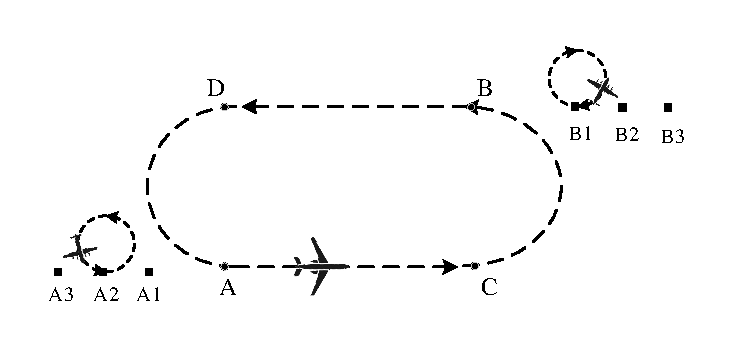
\includegraphics[width=.4\textwidth]{Figures/Figs_Ch15/fig1_1.pdf}}
	\caption{Tanker's path and virtual queue sequence points.}
	\label{fig}
\end{figure}
The design of the tanker's path is shown in Fig. 1, which contains two parts, the straight line refueling section (AC and BD in Fig. 1) and the semi-circular arc section ( $ \stackrel\frown{\rm{AD}} $ and $ \stackrel\frown{\rm{BC}} $ in Fig. 1). Besides, the points A and B are called ``rendezvous point", at which the tanker and receiver rendezvous, the points C and D are called ``separation point", at which the receiver finishes the refueling task and separate from the tanker.

The length and time of the two parts can be determined based on the following three guidelines.
\begin{itemize}
	\item The length of the straight line refueling section is sufficient for one receiver to complete the refueling mission.
	\item Since the semi-circular arc section is not suitable for refueling, it is hoped that the tanker can fly through this section in the shortest time.
	\item The  tanker flies horizontally in a straight line at a constant velocity $ v_{t} $ during the refueling section.
\end{itemize}
So the time of the refueling section is 
\begin{equation}
{t}_{\text{internal}}=(t_{\text{refueling}}+t_{\text{operation}}) \times \gamma
\end{equation}
where $ {t}_{\text{refueling}} $ is the time that the receiver's fuel from empty to full, $ {t}_{\text{operation}} $ is the time for the docking and separation of the receiver and the tanker in the refueling process and the item $ {\gamma} $ is a margin.
And the length is 
\begin{equation}
{L}=v_{t}\times{t}_{\text{internal}}
\end{equation}
For the semi-circle arc section, since it is not suitable for refueling, we want the tanker to fly over in the shortest time, so the radius at maximum hovering angular rate is  
\begin{equation}
{R}=\dfrac{v_{t}^{2}}{g\sqrt{2K_{\text{T}}-2}}
\end{equation}
where $ {g} $ is the gravitational acceleration and $ {K}_{\text{T}} $ denotes dimensionless thrust factor. Then we can obtain the time of the second part
\begin{equation}
{t_{\text{arc}}}=\dfrac{\pi \times v_{t}}{g\sqrt{2K_{\text{T}}-2}}.
\end{equation}

This paper considers the refueling situation when a group of receivers arrive at the refueling area with a small time interval, i.e., the receivers need a specific area to wait for other receivers to finish refueling. For such a purpose, we design virtual queue sequence points (A1,A2,A3... and B1,B2,B3...) near rendezvous points A and B as shown in Fig. 1. The distance between virtual queue sequence points is determined by the specific parameters of the receiver, which can be represented by
\begin{equation}
{l}=2 \times r+l_{\text{offset}}
\end{equation}
where $ {r} $ is the minimum turning radius of the receiver and $ {l}_{\text{offset}} $ is a compensation term to ensure safety.



\subsection{Refueling Task Procedures}
The procedure of the refueling task described in this paper can be divided into the following steps:
\begin{itemize}
	\item [ 1.] At the beginning of the refueling task, each receiver is assigned a refueling sequence value according to its operational mission or its own status.
	\item [ 2.] The first receiver in the refueling sequence meets the tanker directly, other receivers are assigned virtual queue sequence points, and then fly to these points.
	\item [ 3.] The receivers refuel in sequence, and when the previous receive begins to rendezvous with the tanker, the sequence waiting for refueling moves into position in turn to form a new queue as shown in Fig. 3.
	\item [ 4.] The receiver rendezvous with the tanker at point A or point B, and finish refueling and fly back to the task region at point C or point D.
\end{itemize}
\begin{figure}[htbp]
	\centerline{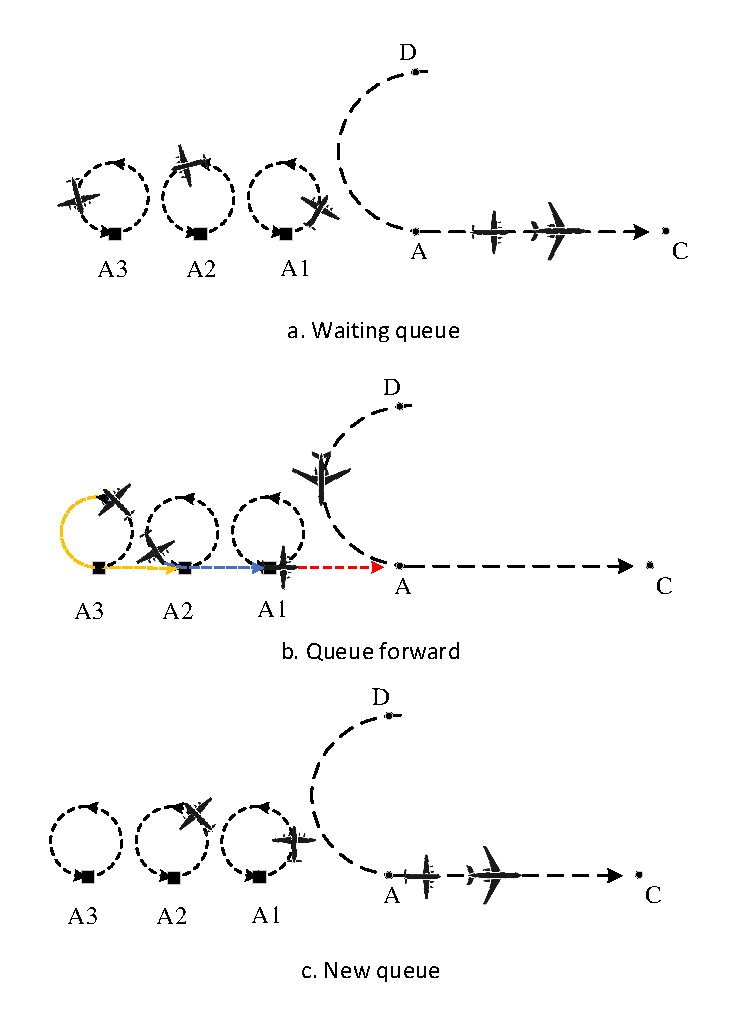
\includegraphics[width=.4\textwidth]{Figures/Figs_Ch15/fig2_1.pdf}}
	\caption{Queue adjustment}
	\label{fig}
\end{figure}


According to the steps above, the refueling mission of a single receiver can be divided into five phases:``mission", ``cruise", ``waiting", ``rendezvous", ``refueling".
\begin{itemize}
	\item \textit{Mission phase}: The receiver performs task.
	\item \textit{Cruise phase}: The receiver flies to the assigned virtual point.
	\item \textit{Waiting phase}: The receiver is staying in the waiting queue.
	\item \textit{Rendezvous phase}: The receiver rendezvouses with the tanker from the waiting point.
	\item \textit{Refueling phase}: The receiver docks with the tanker and refuels.
	
\end{itemize}
\section{Problem Analysis}

To achieve the minimum time consumption, in the five phases, the time of the ``refueling phase" cannot be changed. The time of the rest four phases is related to the assigned virtual points. In this study, the assignment strategy can be described as the following $ \{ 0, 1 \} $ matrix form:
\begin{equation}
\textbf{S}=\left [ \begin{matrix}
s_{11} & \cdots  &  s_{1m}\\
\vdots  & \cdots  & \vdots\\
s_{n1} & \cdots &   s_{nm}
\end{matrix} \right ]  
\end{equation}
where $ s_{ij} =1$ means the $ j $th virtual point is assigned to the $ i $th receiver, otherwise it is equal to $ 0 $ and $ n $ is the amount of the receivers and $ m $ is the amount of the virtual queue sequence points. And any receiver is uniquely assigned to one point, i.e.,
\begin{equation}
\sum_{i} s_{i,j} =1.
\end{equation}
Obviously, the assignment strategy depends on the shortest travel time or shortest travel distance for each receiver to reach the virtual queue sequence point. Because of the presence of the refueling sequence and the constraints of the tanker's path, the shortest travel time or shortest travel distance is related to the following constraints. 
\begin{itemize}
	\item [ 1.] \textbf{Tanker's Path Constraints}:
	The design of the tanker's path require the receiver should rendezvous with the tanker at point A or point B, and leave at point C or point D. If the receiver misses the timing, it should wait until the next time the tanker pass the points.
	\item [ 2.] \textbf{Task Constraints}: 
	The range of time intervals $ \triangle {t}_{\text{internal}} $ between two adjacent receivers arriving at the refueling area is relative small, which is $ {T}_{\text{tanker}}=2 \times({t}_{\text{internal}}+{t_{\text{arc}}}) \ge \triangle {t}_{\text{internal}} \ge 0 $. Besides, the receivers need to be refueled in sequence, which is determined at the beginning of the refueling task based on the tasks performed by each receiver and its own status. The receiver of the first order is supposed to rendezvous with the tanker directly at point A.
	
\end{itemize}

By calculating the minimum time $ t_{ij} $ for each UAV $ i $ to navigate to the assigned virtual point of the refueling $ j $, the shortest rendezvous matrix for the planned path of the tanker and the receiver can be obtained
\begin{equation}
\textbf{T}=\left [ \begin{matrix}
t_{11} & \cdots  &  t_{1m}\\
\vdots  & \cdots  & \vdots\\
t_{n1} & \cdots &   t_{nm}
\end{matrix} \right ]  .
\end{equation}

Given a strategy $ \textbf{S} $, the overall time for the refueling task can be obtained as
\begin{equation}
{T}_{\text{total}}={\rm{vec}}(\textbf{T})^{\rm{T}} {\rm{vec}}(\textbf{S}).
\end{equation}
where $ \rm{vec} $ represents  .
The problem of optimal aerial refueling time assignment can be described as an Integer Linear Programming (ILP) problem
\begin{equation}
\min_{s_{ij}}  \ {\rm{vec}}(\textbf{T})^{\rm{T}} {\rm{vec}}(\textbf{S})
\end{equation}
subject to:
\begin{equation}
\begin{cases}
\textbf{A}  {\rm{vec}}(\textbf{S})= \mathbf{b }\\
s_{ij} \in \left \{ 0,1 \right \}
\end{cases} 
\end{equation}
where $ \textbf{S}=[s_{ij}] \in \mathbb{Z}^{n \times m}$ represents the assignment strategy, $ \textbf{b}=[1\ 2\ \dots \ n]^{\rm{T}} $, $ \textbf{A}=(\textbf{I}_{n \times n}\otimes[1\ 2\ \dots \ m]^{\rm{T}}) $ and $ \otimes $ is the Kronecker product. Eq. (11) comes from Eqs. (6) and (7).

The ILP is widely used to solve Traveling salesman problem (TSP) , Petri net analysis problem, and project scheduling problem \cite{b8}, etc. The solution methods for the ILP problem include branch and bound, heuristic search and tangent plane method. Among them, the branch and bound algorithm is simple, straightforward, and fast on average \cite{b8}, and a lot of commercial software has been developed. Therefore, this algorithm is used in this paper. The essence of the branch and bound method is to solve the value of the objective function of each node while enumerating the nodes, and stop the enumeration of this branch if the value can be determined to be the optimal solution on that branch. So it is necessary to find when to bound. The problem of the refueling task in this paper can be divided into two sub problems:
\begin{itemize}
	\item [ 1.]\textbf{Task Assignment.} Design appropriate bound criteria to solve the ILP problem (10),(11) using the branch and bound method.
	\item [ 2.]\textbf{Velocity Planning.} Design velocity controller for each receiver to allow the receiver to move safely and orderly through the designed waiting queue and rendezvous with the tanker.
\end{itemize}
\section{Virtual target points assignment and Queue Waiting Strategy Design}
In this section, a bound criterion is proposed to solve the ILP problem. The choice can be considered as the overall optimal solution under the condition of having refueling aircraft path restrictions. 
\subsection{Priority initialization}\label{AA}
The priority initialization function contains two parts, the one is determined by human-specified task priorities, the other is the receiver's states. So the function can be represented as
\begin{equation}
pri{(i)}=\begin{cases}
h{(i)} \\
val_{i,\text{initial}} +d_{i,A}/k 
\end{cases}
\end{equation}
where $ h{(i)} $ is artificially established, and $ val_{i,\text{initial}} $ is the initial fuel of the receiver at the beginning of the task, $ d_{i,A} $ is the distance between the receiver and point A, $ k $ is the fuel efficiency of the receiver per kilometer, so the second part is the receiver's fuel when it arrives point A.
\subsection{Virtual Target Point Assignment}
Because of the existence of the refueling sequence, the branching order of the branch and bound method is already known, and at the same time, due to the design of the tanker path, as long as the refueling time at each branch node is guaranteed to be the shortest, then the total refueling time should be the least.

The virtual target point available to the current receiver is determined by the distribution of receivers ahead in the refueling order. Because the first receiver will directly merge with the tanker at point A at the beginning of the refueling mission, its situation is rather special, so we will first discuss the target point assignment of the first two receivers.
\begin{figure}[htbp]
	\centerline{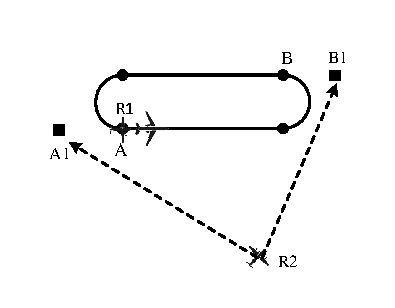
\includegraphics[width=.25\textwidth]{Figures/Figs_Ch15/fig3.pdf}}
	\caption{Target point option for the first two receivers}
	\label{fig}
\end{figure}

As shown in Fig. 4, R2 (the 2nd receiver) has two optional virtual target points A1 and B1 due to the task constraints. Nowadays, studies generally consider calculating the paths to reach A1,B1, and which one is shorter will be used as the target point. However, for the context of this thesis, when R2 reaches point B1, although the path is shorter, the tanker may have already flown past point B. Then R2 needs to wait for the next time that the tanker passes point B. At this time, although it takes longer to reach point A, it can arrive before the tanker reaches point A. R2 obviously chooses target point A1.
Since the coordinates of the virtual point and the position of R2 are known, the  arrival time of R1 (the 1st receiver) to point A and the arrival time of R2 to B1 can be calculated and the time interval can be obtained, i.e.,
\begin{equation}
\begin{split}
\triangle {t}^{\rm{B}}_{{1,\rm{2}}}=t_{2,\rm{B1}}-t_{1,\rm{A}} 
\end{split}
\end{equation}
where $ t_{2,\rm{B1}} $ is the arrival time of R2 to B1 and $ t_{1,\rm{A}} $ is the arrival time of R1 to point A.
So we first compare $ \triangle {t^{\rm{B}}}_{\rm{1,2}} $ with $ {T}_{\text{tanker}} /2$, if $ \triangle {t}^{\rm{B}}_{\rm{1,2}}<{T}_{\text{tanker}} /2 $, the target point of R2 is B1. Otherwise, the target point of R2 is A1. 

For more general situations, the judgment conditions are more complex. As shown in Fig. 5, for a receiver Ri (the $ i $th receiver), it has four optional virtual target points A2, A3, B1, B2, the reason can be found in Fig. 6. In Fig. 6(a), if the previous receiver is assigned to refuel at point B, Ri should take  the assignment to A3 into account, but also the case of A2.It happens when Ri arrives at A2, the previous aircraft has already left for refueling or moved forward as seen in Fig. 6(b). This situation is usually caused by the relatively large time interval between the arrival times of the receivers. When the receiver arrives at the target point, the receiver at the head of the same queue have already flown from the waiting area to the rendezvous point, so the queue will move forward one step as a whole.

First, Ri needs to consider whether the previous receiver is assigned to queue A or queue B. If it is queue A, Ri should consider B1, B2 first, otherwise it should give priority to A2,A3 in Fig. 5. Then check if there is a queue forward for those assigned in the same queue, finally select the target point.

\begin{figure}[htbp]
	\centerline{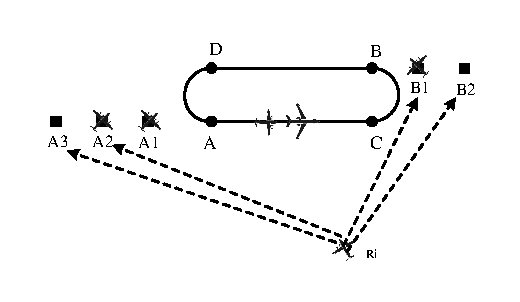
\includegraphics[width=.35\textwidth]{Figures/Figs_Ch15/fig4.pdf}}
	\caption{Target points options for formal receivers}
	\label{fig}
\end{figure}
\begin{figure}[htbp]
	\centerline{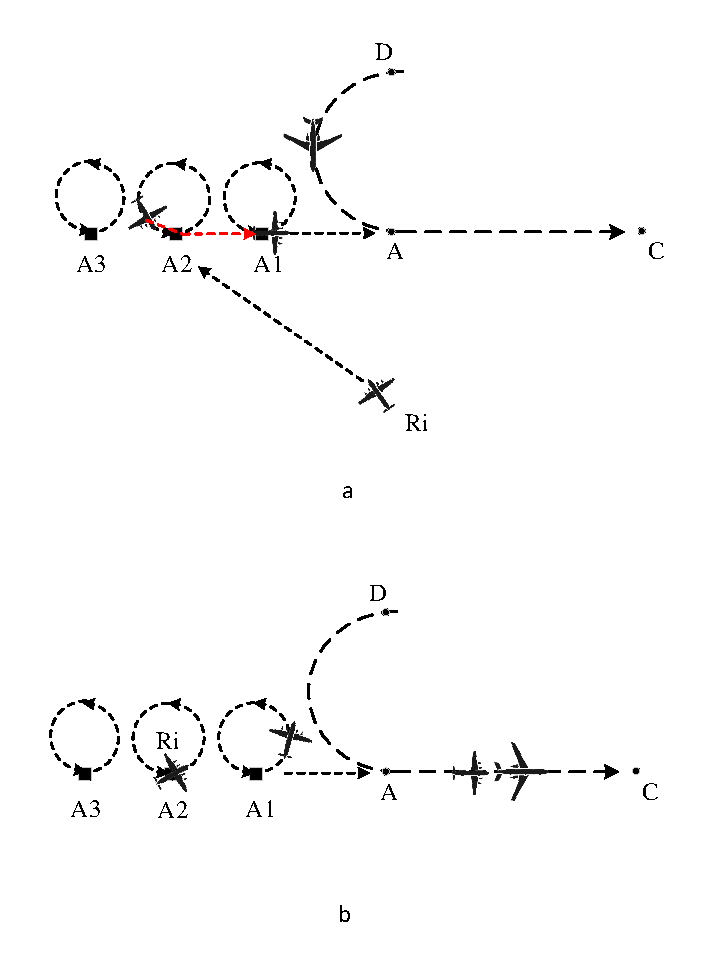
\includegraphics[width=.35\textwidth]{Figures/Figs_Ch15/fig5.pdf}}
	\caption{Ri considers the case of A2}
	\label{fig}
\end{figure}

\begin{algorithm}[!h]
	\caption{Assignment}%????
	\begin{algorithmic}[1]%???????
		\REQUIRE $ {T}_{\text{tanker}} $,  coordinates of virtual target points near point A in set $ \mathcal{A} $, coordinates of virtual target points near point B in set $ \mathcal{B} $, and $   \mathcal{A} _{i} $ and $  \mathcal{B}_{j} $ represent the $ i $th and $ j $th element in set $ \mathcal{A} $ and $ \mathcal{B} $.
		\ENSURE $ \textbf{S} $
		
		Let set $ \mathcal{C} $ to record the receivers that will rendezvous with the tanker at point A, set $ \mathcal{D} $ at point B. Let $ numA $ to record number of occurrences of situation shown in Fig. 6 at point A, and $ numB $ at point B.
		\FOR{$i=3$ to $n$}
		\IF{ $i-1\in \mathcal{C}$}
		\STATE {$ j $ $= \rm{max}({\mathcal{D}}) $ } 
		
		\STATE {calculate $ \triangle t^{\rm{B}}_{i,{j}}=t_{i,{\rm{B}}j}-t_{i-1,\rm{A}} $}
		\STATE {$k= \rm{min}({\mathcal{D}}) $$ +numB $}
		\STATE {compare  $k $th receiver's beginning refueling time $ t_{\text{Bqueuehead}} $ with  $ t_{i,{\rm{B}}j} $} 
		\IF{ $\triangle t^{\rm{B}}_{{i,j}}<{T}_{\text{tanker}}/2$ and $ t_{{i,{\rm{B}}j}}>t_{\text{Bqueuehead}} $ }
		\STATE {add $ i $ to $ \mathcal{D} $ and $ i $th receiver is assigned to $ \mathcal{B}_j $ }
		\ELSIF{$\triangle t^{\rm{B}}_{{i,j}}< {T}_{\text{tanker}}/2$ and $ t_{i,{\rm{B}}j}<t_{\text{Bqueuehead}} $}
		\STATE {add $ i $ to $ \mathcal{D} $ and  $ i $th receiver is assigned to $ \mathcal{B}_{j+1} $  }
		\ELSIF{$\triangle t^{\rm{B}}_{i,j}> {T}_{\text{tanker}}/2$ }
		\STATE { $l     = \rm{max}({\mathcal{C}}) $ }
		\STATE { $m= \rm{min}({\mathcal{C}}) $$ +numA $}
		\STATE {compare  $ m $th receiver's beginning refueling time $ t_{\text{Aqueuehead}} $ with  $ t_{i,\text{A}l} $} 
		\IF{$ t_{i,\text{A}l}>t_{\text{Aqueuehead}} $ }
		\STATE {add $ i $ to $ \mathcal{C} $ and $ i $th receiver is assigned to $ \mathcal{A}_{l+1} $ }
		\ELSIF{$ t_{i,\text{A}k}<t_{\text{Aqueuehead}} $  }
		\STATE {add $ i $ to $ \mathcal{C} $ and $ i $th receiver is assigned to $ \mathcal{A}_{l} $ }
		\ENDIF
		\ENDIF
		\ENDIF
		
		\ENDFOR
	\end{algorithmic}
\end{algorithm}


\subsection{Design of the Velocity Controller}\label{SCM}
In order to ensure safe and efficient refueling, the following specifications should be followed when receivers are in the queue:
\begin{itemize}
	\item [ 1.] The asion whether to move forward or not when a receiver begins to rendezvous with the tanker.
\end{itemize}

The corresponding reasons are as follows:


For rules 1 and 2 mentioned above, in actual combat, to avoid danger, the planned paths are often required to cross as few or even no crossings as possible. So each aircraft has to ensure that it flies a full circle before any other action is taken as shown in Fig. 6.

On the other hand, there is a limit to the velocity of the receiver, and we cannot guarantee that each receiver will move forward one step every time when a receiver begins refueling under the above-mentioned path-free condition, which means that the receiver needs to make a decision whether to move forward or not every time to decide its velocity. So the velocity limit may lead to a situation as shown in Fig. 7. It can be seen that due to the velocity limitation, the receiver at point A2 will not be able to fly to point A and fly another full circle before  next time tanker arrives at point A.  This scenario has an impact on the previous algorithm, and the target points available to each receiver change accordingly, as the queue may not move or move two points when the receiver at the front of the queue starts refueling. When the receiver on A2 starts refueling, the receiver on A3 will first consider flying to A1 instead of A2. 
For the example of the previous assignment point in queue A, the corresponding assignment logic is shown in \textbf{algorithm 1}.
\begin{figure}[htbp]
	\centerline{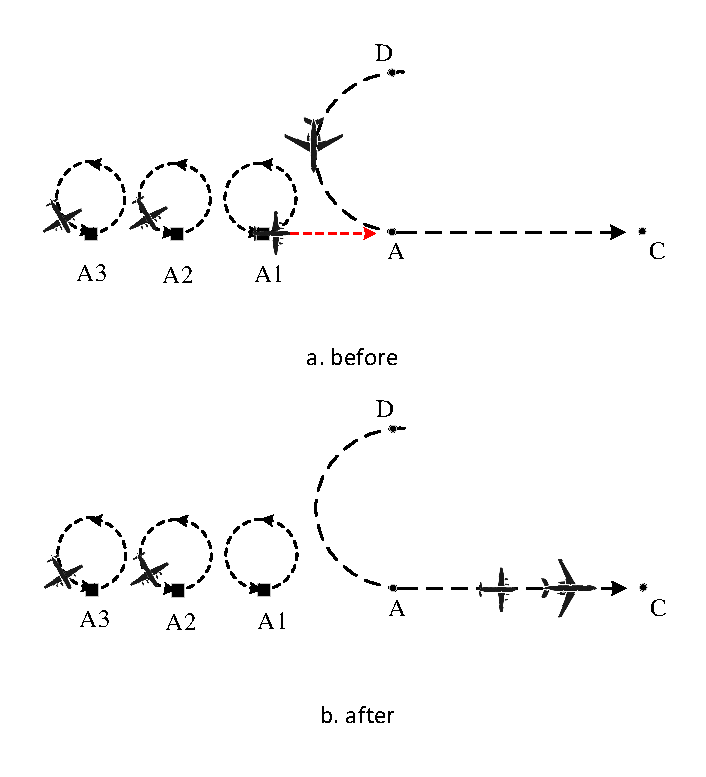
\includegraphics[width=.4\textwidth]{Figures/Figs_Ch15/Fig7.pdf}}
	\caption{Queue position change considering velocity limit}
	\label{fig}
\end{figure}


\section{Simulation and Results}



To verify the efficiency of the designed algorithm, a simulation model is build in MATRLAB/Simulink using the ``Stateflow" toolbox. The state of each of receivers and the corresponding transition conditions are the same as those discussed above as seen in Fig. 8. In Fig. 8, for example, the ``TC1" condition means that the receiver's fuel has been in an unhealthy state.
\begin{figure}[htbp]
	\centerline{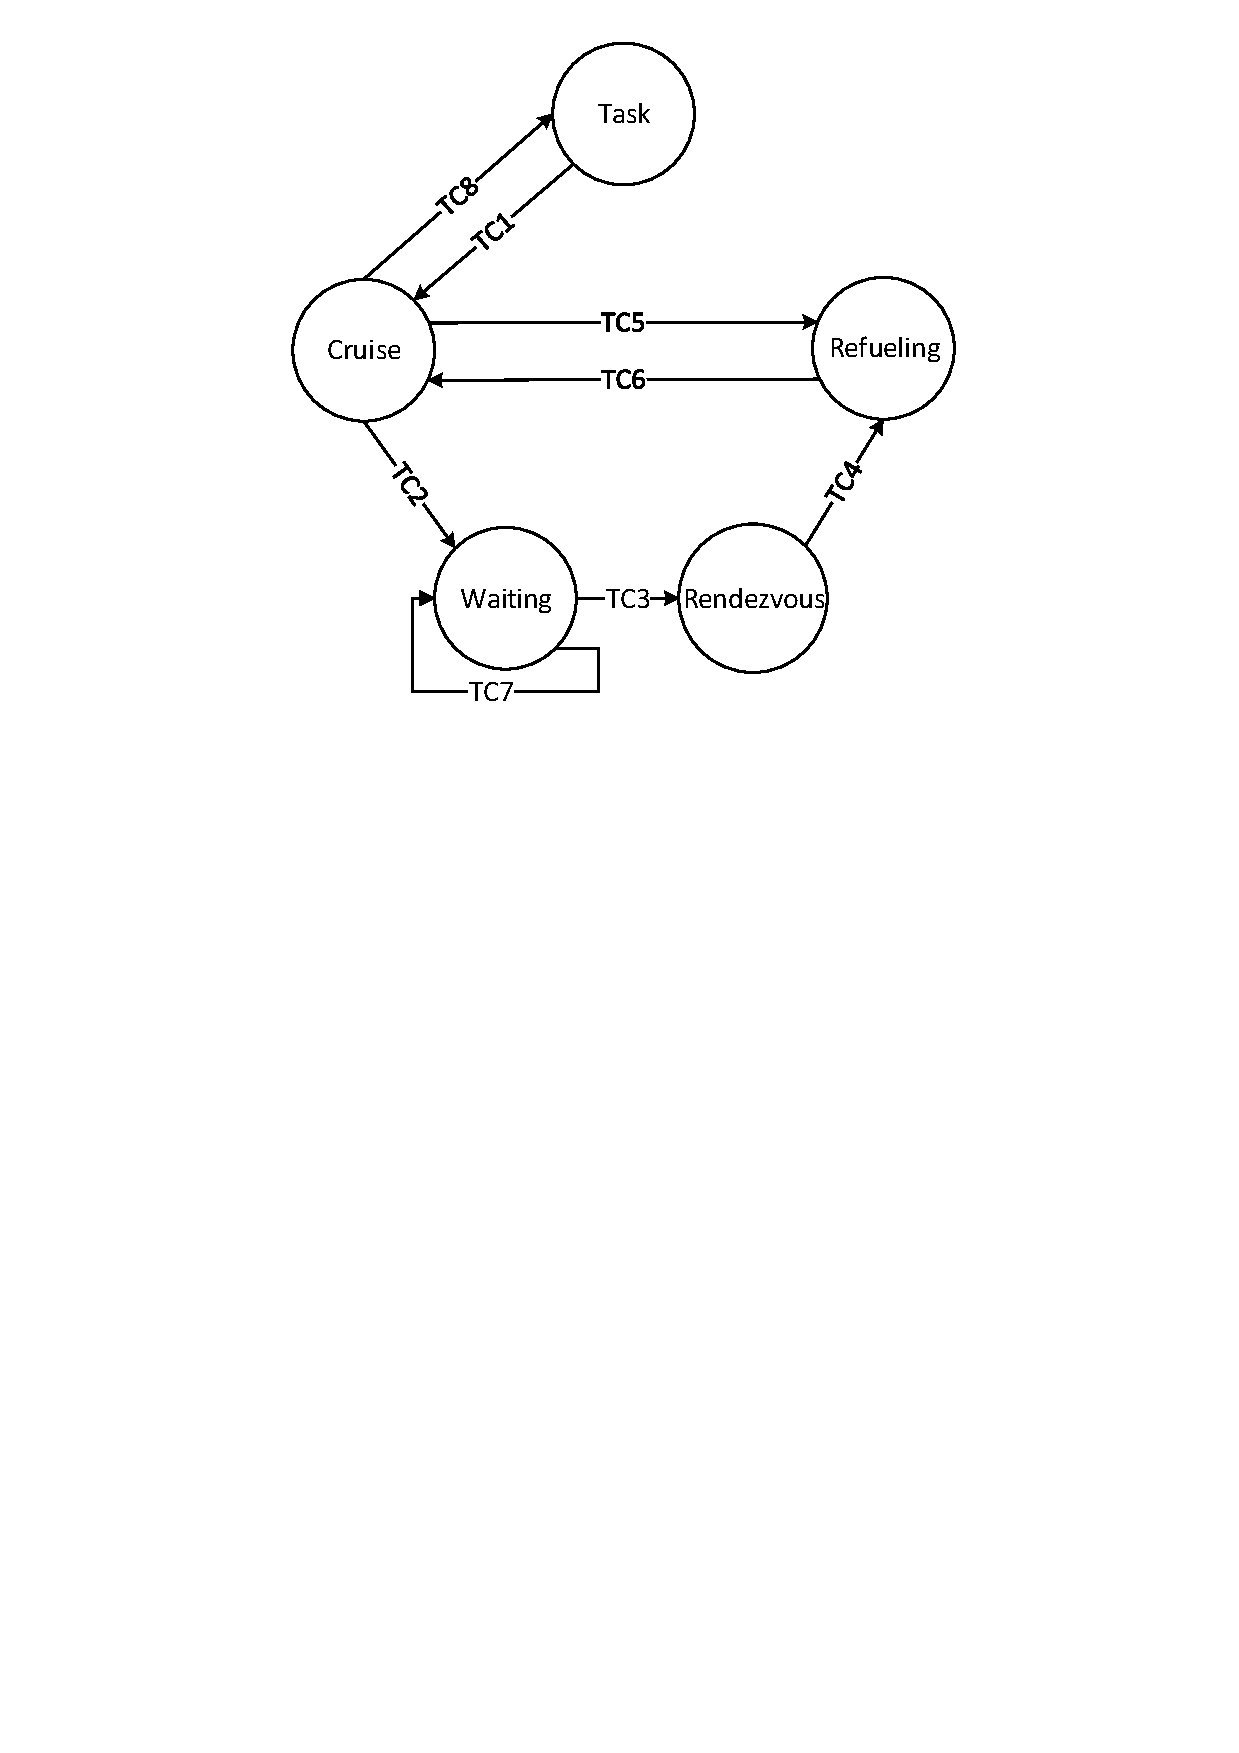
\includegraphics[width=.3\textwidth]{Figures/Figs_Ch15/fig8.pdf}}
	\caption{Finite state machine for receivers}
	\label{fig}
\end{figure}


Here, two indexes are defined, namely, the minimum oil volume of the receivers  and the average oil volume of the receivers at the start of refueling. Due to different assignment strategies under the same initial conditions, each UAV starts refueling with a different amount of fuel. The initial fuel volumes of 11 receivers are set between 1400 and 1600 randomly. Simulations are performed and the values of the two indexes are recorded according to different allocation strategies, and the results are shown in Fig. 9. The first seven simulations are randomly assigned waiting points according to the refueling order, and the eighth simulation is a refueling task according to the assignment strategy proposed in this paper. It can be observed that, under the same starting conditions, the assignment strategy proposed in this paper can ensure the highest oil volume when the receiver starts refueling. Besides, the trajectory of UAVs can be found in Fig. 10, here, we assume that during the ``mission" phase the UAV takes a roundabout way, under the velocity designed before. It can be observed that the trajectories of each UAVs are not repeated, and all flying complete circles in the waiting area.



\begin{figure}[htbp]
	\centerline{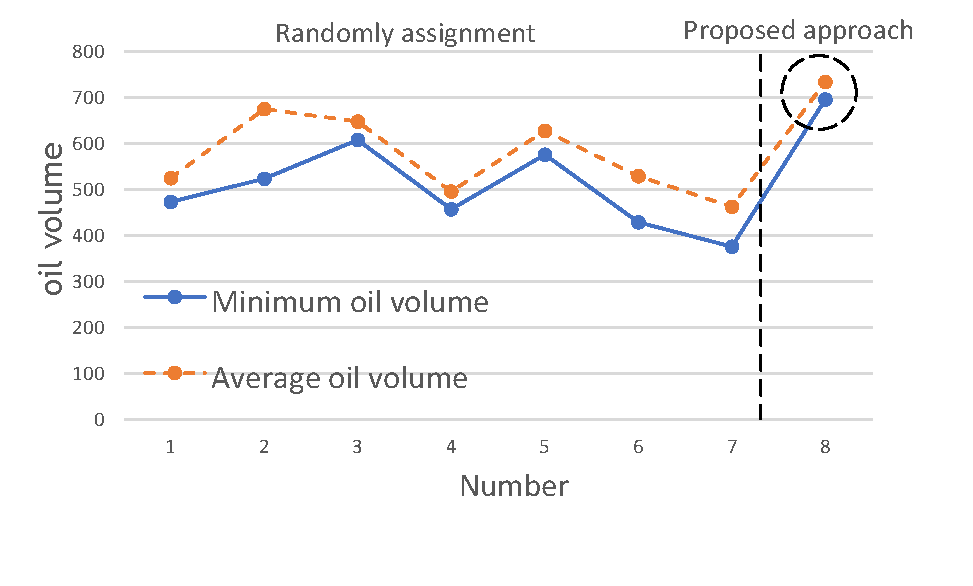
\includegraphics[width=.5\textwidth]{Figures/Figs_Ch15/fig10.pdf}}
	\caption{Comparison with Randoml assignments}
	\label{fig}
\end{figure}
\begin{figure}[htbp]
	\centerline{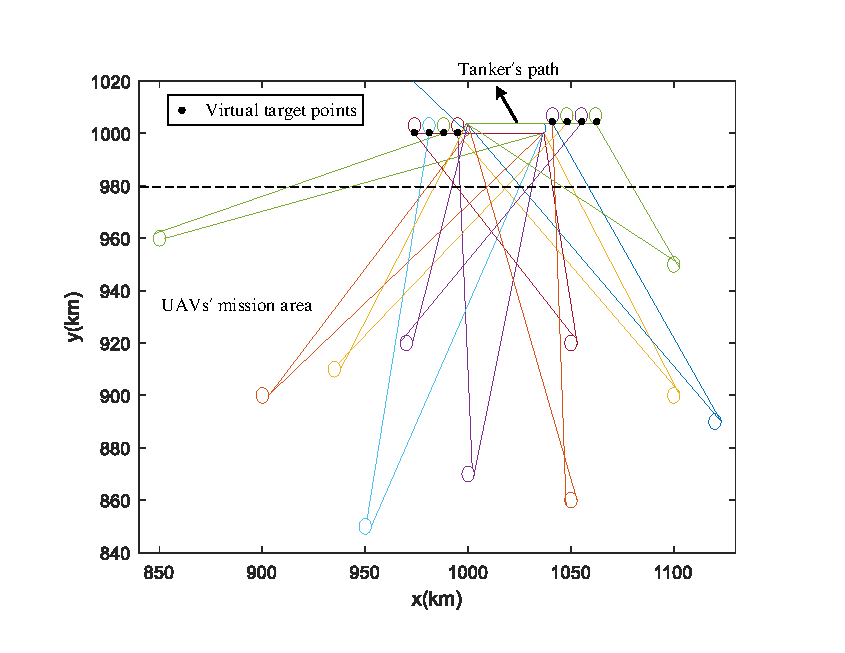
\includegraphics[width=.5\textwidth]{Figures/Figs_Ch15/fig9.pdf}}
	\caption{UAVs trajectory}
	\label{fig}
\end{figure}


\section{Chapter Summary}
This paper proposed a novel whole  strategy for intensive refueling task of multiple receivers, which contains the design of the tanker's path and virtual queue sequence points. Based on the strategy, an target points assignment algorithm based on the branch and bound method are proposed and velocity planning is designed when the receivers waiting in the queue to get the minimum refueling time.
Simulations results show that the proposed method ensures efficient refueling for multiple receivers. In future studies, consider abnormal situations, such as refueling docking failure, decide whether to continue refueling or go back to the waiting area. Furthermore, more accurate path planning will be considered, including dynamics constraints and obstacle avoidance.